\begin{exo}
  \donnee{Considérons deux variables aléatoires X et Y dont les fonctions de densité $f_x$ et $f_y$ se trouvent dans la Figure1. En n'effectuant aucun calcul, l'écart type de X est-t-il plus grand que l'écart type de Y ?}
  \begin{center}
  	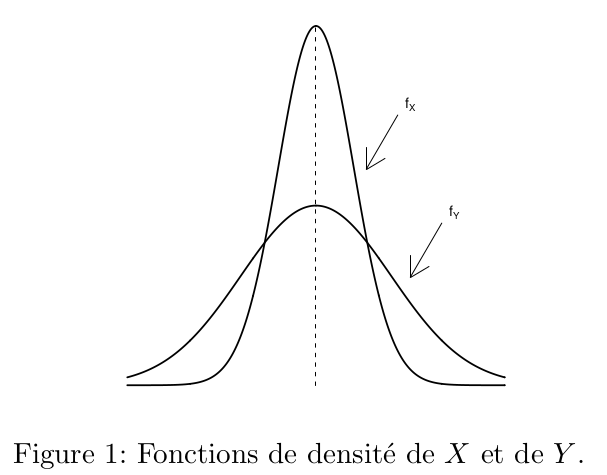
\includegraphics[width=10cm]{ex5.png}
  \end{center}
	\begin{center}
		Non, on peut constater que la courbe $f_y$ est plus applatie (plus grande dispertion). Donc $\sigma_x < \sigma_y$
	\end{center}
\end{exo}
